% Time Windows for Free -- ICCS 2027 submission draft (Springer LNCS).
% The text was drafted with AI assistance (see "Use of AI tools" at the end); the author must
% read, verify and own every sentence before submitting. Open items: paper/ROADMAP.md.
%
% Numbers: every number in a table or in the text is copied from results/; comments name the
% source file. Run `python3 paper/check_numbers.py` after editing: it fails if a decimal,
% percentage or k/m count outside a comment is not in results/*.txt.
%
% Build: `tectonic main.tex` (or pdflatex + bibtex on Overleaf); `sh arxiv.sh` makes the arXiv zip.
\documentclass[runningheads]{llncs}
\usepackage[T1]{fontenc}
\usepackage{graphicx}
\usepackage{amsmath,amssymb}
\usepackage{booktabs}
\usepackage[hidelinks]{hyperref}
\graphicspath{{../figures/}{figures/}{./}}   % repo layout, Overleaf with a figures/ folder, or flat
\renewcommand{\topfraction}{0.9}             % let floats share pages with text instead of
\renewcommand{\textfraction}{0.1}            % leaving half-empty float pages
\renewcommand{\floatpagefraction}{0.8}

% Macros and abstract shared by main.tex (Springer LNCS) and elsevier.tex (Elsevier CAS).
\newcommand{\Popt}{P(\mathrm{opt})}
\newcommand{\Pvalid}{P(\mathrm{valid})}
\newcommand{\Pontime}{P(\text{on time})}
\newcommand{\LB}{\mathit{LB}}
\newcommand{\iv}[1]{\bigl[\,#1\,\bigr]}   % Iverson bracket: 1 if #1 holds, else 0
\newcommand{\repourl}{\url{https://github.com/Mithilbatra/time-windows-for-free}}

% source for the numbers: results/qaoa_grid_summary.txt, results/sa_up_summary.txt, results/pruning_large.txt
\newcommand{\theabstract}{%
QUBO encodings of the travelling salesman problem with time windows (TSPTW) usually enforce
the windows with slack variables, which multiplies the number of qubits and two-qubit gates. We
bound every customer's earliest possible service start at every tour position with a dynamic
programme and turn the bounds into penalties. The resulting encoding, E1, needs no qubits or
two-qubit terms beyond those of the window-free position encoding and provably never penalises
a feasible route; a look-ahead variant, E1+C, prunes more for a few percent more two-qubit
terms. In exact QAOA simulation with an XY mixer on three to five customers, E1+C raises the
probability of sampling the optimal route over a window-free encoding at every depth, by 0.094
to 0.217 at depth 12. Under simulated annealing, E1 and E1+C outperform the slack-qubit encoding
of Salehi et al.\ and a slack-free unbalanced-penalization variant of it with far fewer qubits.
Over all routes of instances with up to nine customers, E1 penalises 68.8--85.2\% of the late
routes and, unlike a recent heuristic penalty, never an on-time one.}
   % macros and the abstract; the body is in body.tex

\begin{document}

\title{Time Windows for Free: A Sound, Ancilla-Free Time-Window Encoding for QAOA on the TSP with Time Windows}
\titlerunning{Time Windows for Free}
\author{Mithil Batra}
\authorrunning{M. Batra}
\institute{Department of Computer Science and Engineering,\\ National Institute of Technology Delhi,
Delhi 110036, India\\ \email{mithil.batra05@gmail.com}}

\maketitle

\begin{abstract}
\theabstract
\keywords{QAOA \and TSP with time windows \and QUBO \and XY mixer \and Penalty methods}
\end{abstract}

% The paper's body, shared by main.tex (Springer LNCS) and elsevier.tex (Elsevier CAS).
% ---------------------------------------------------------------------------------------------
\section{Introduction}\label{sec:intro}

The travelling salesman problem with time windows (TSPTW) asks for the shortest closed tour
that starts at a depot, visits each of $n$ customers once and serves customer $j$ inside its
time window $[e_j,l_j]$, waiting if it arrives early. Windows make routing practical, and
they are what makes the TSPTW awkward to encode for a quantum optimiser.

Variational algorithms such as the quantum approximate optimisation algorithm
(QAOA)~\cite{farhi2014qaoa,hadfield2019qaoa} minimise a diagonal cost Hamiltonian, so a
routing problem must first be written as a quadratic unconstrained binary optimisation (QUBO)
problem. For the plain TSP the standard choice is the position encoding~\cite{lucas2014ising}:
one binary variable per (customer, position) pair, $n^2$ in all once the depot is fixed, with
quadratic penalties for the one-hot constraints and a quadratic distance term. Time windows do
not fit this pattern. Whether customer $j$ is on time at position $k$ depends on the arrival
time there, which depends on the whole prefix of the tour, and the window is an inequality.

Existing TSPTW QUBOs therefore add variables: they hold arrival or waiting times in binary
registers and turn each window inequality into an equality with binary slack
variables~\cite{papalitsas2019qubo,salehi2022unconstrained}. The corrected edge-based QUBO of
Salehi et al.~\cite{salehi2022unconstrained} needs up to $n^3-2n^2+3n+3n\delta$ qubits, where
$\delta$ is the number of bits per time value; on our instances that is 60.5 to 165.7 qubits
for three to five customers, against 9 to 25 for the position encoding
(Table~\ref{tab:resources}). Every slack bit also enters squared penalty terms, so the number
of two-qubit terms per QAOA layer grows faster still.

We take a different route, borrowed from exact classical algorithms for the TSPTW, which use
the windows to rule out states and transitions before they search~\cite{dumas1995optimal}.
Before building the QUBO we compute, by a dynamic programme, a lower bound $\LB_{j,k}$ on the
time at which customer $j$ can be served if it is the $k$-th stop. If the bound already misses
$j$'s window, the variable $x_{j,k}$ is penalised; if going from $u$ at position $k$ to $j$ at
position $k+1$ must miss $j$'s window, that pair of variables is penalised. These pairs are
pairs the distance term already couples, so the encoding, which we call E1, adds no qubits and
no two-qubit terms. Because the bound is a lower bound, no feasible route is ever penalised:
every feasible route keeps its tour cost as its energy (Lemma~\ref{lem:sound}). The price is
completeness, since some infeasible routes stay unpenalised and compete on cost alone. A
variant with a two-step look-ahead, E1+C, penalises more of them at the cost of new two-qubit
terms. Our contributions are:
\begin{itemize}
  \item E1, a time-window penalty built from cumulative earliest-arrival bounds that needs no
        extra qubits or two-qubit terms, with a proof that it never penalises a feasible route,
        and E1+C, a sound look-ahead variant (Sect.~\ref{sec:method});
  \item a classical pruning analysis by full route enumeration up to nine customers, including
        the penalty of Rezk and Gora~\cite{rezk2026gnn}, the closest prior work
        (Sect.~\ref{sec:res-pruning});
  \item a comparison under simulated annealing with the slack-qubit encoding of Salehi et al.\ and
        a slack-free unbalanced-penalization variant of it, with every encoding's weights
        tuned the same way on separate instances, and a window-tightness study
        (Sect.~\ref{sec:res-sa});
  \item exact simulation of QAOA with X and XY mixers to depth 12 on fresh instances, with
        paired statistics (Sect.~\ref{sec:res-qaoa}).
\end{itemize}

% ---------------------------------------------------------------------------------------------
\section{Related Work}\label{sec:related}

\paragraph{TSPTW as a QUBO.} Papalitsas et al.\ gave the first QUBO for the
TSPTW~\cite{papalitsas2019qubo}, assuming that every window opens at time zero. Salehi, Glos
and Miszczak~\cite{salehi2022unconstrained} reported a flaw in it and gave a corrected
edge-based QUBO in which binary registers hold waiting times and slack variables close each
window inequality, alongside a node-based higher-order model and an ILP-based QUBO, and ran them
on a D-Wave annealer. Their edge-based QUBO is our baseline E2. They also bound the arrival time
at the $i$-th position from below (their Eq.~18), with one bound per position for all cities and
without waiting, and use it only to size the slack registers; a footnote suggests sharpening it
with shortest paths from the depot. Our $\LB_{j,k}$ carries this idea further: it is specific to
each city, includes waiting, extends only prefixes that are themselves on time, and is used as
the penalty itself, which removes the slack variables altogether.

\paragraph{Closest work.} Rezk and Gora~\cite{rezk2026gnn} encode the capacitated vehicle
routing problem with time windows (CVRPTW) for a quantum annealer, using the position encoding
of Borowski et al.~\cite{borowski2020new} and graph coarsening for larger instances. Their
time-window penalty, whose exact form is given in their code~\cite{rezk2026code}, has three
tiers built on one earliest-arrival value per customer, the same at every step,
\[ \hat e_j = \max\bigl(e_j,\; e_0 + d_{0j}\bigr): \]
a check at the first step, a hard and a graded soft penalty on consecutive pairs, and a
look-ahead from step $k$ to $k+2$. E1 differs in four ways: its bound grows with the position,
so it reflects cumulative travel time; its single-variable terms apply at every position; it is
sound for any travel times, whereas their hard tiers rely on the triangle inequality and their
soft tier can penalise a feasible route, a reasonable heuristic for annealing with classical
repair that nevertheless moves the ground state; and it stays on existing couplings, whereas
their look-ahead needs new two-qubit gates in a gate-model circuit. E1+C uses a look-ahead of
their kind built on $\LB$, which keeps it sound.

\paragraph{Other quantum approaches to routing with windows.} Holliday et
al.~\cite{holliday2025advanced} solve the TSPTW and the CVRPTW with a hybrid
constrained-quadratic solver and classical repair, and observe that window feasibility drops as
instances grow, one reason we report feasibility alongside optimality. Harwood et
al.~\cite{harwood2021formulating} compare several formulations of routing with time windows by
QUBO-hardness metrics and in simulated VQE, QAOA and ADMM runs. Leonidas et
al.~\cite{leonidas2023qubit} study qubit-efficient variational algorithms for the vehicle
routing problem with time windows on NISQ processors.

\paragraph{QAOA for routing without windows.} QAOA results for vehicle routing depend on the
optimiser, depth and initialisation~\cite{azad2023solving}, and on hardware penalty scaling
decides feasibility~\cite{azfar2025quantum}. Mixers for the TSP have been
compared~\cite{qian2023comparative}, XY mixers, which keep one-hot constraints
satisfied~\cite{hadfield2019qaoa,wang2020xy}, combined with warm starts~\cite{docarmo2025warm},
and the search space reduced with an edge-based encoding~\cite{kallerimadhu2025edge}. None of
these handle time windows.

\paragraph{Alternatives to slack variables.} Unbalanced
penalization~\cite{montanezbarrera2024unbalanced} replaces the slack variables of an inequality
by a linear-plus-quadratic penalty; we apply it to Salehi et al.'s window inequalities as a
second baseline, E2-UP. Liu et al.~\cite{liu2024comparison} compare penalty, dephasing and
Zeno-based constraint encodings for QAOA, and binary encodings of the TSP trade qubits for
circuit depth~\cite{glos2022space}. Ayodele~\cite{ayodele2022penalty} gives static rules for
penalty weights in permutation QUBOs; we tune the weights instead, for every encoding alike.
Finally, Soulignac~\cite{soulignac2026beware} argues that the classical TSPTW benchmark sets no
longer represent hard instances; at the sizes a simulator allows we generate instances with
Salehi et al.'s protocol.

% ---------------------------------------------------------------------------------------------
\section{Method}\label{sec:method}

\subsection{Position Encoding with a Fixed Depot}\label{sec:encoding}
A route starts at the depot $0$, visits customers $1,\dots,n$ once each and returns. Travel
from $u$ to $v$ takes time $d_{uv}$, which is also its cost; as in~\cite{salehi2022unconstrained},
service times are folded into $d$. Customer $j$ must be served inside $[e_j,l_j]$, the vehicle
waits if it arrives early, and it leaves the depot at $e_0$ and must be back by $l_0$. With the
depot fixed at position $0$, the position encoding~\cite{lucas2014ising} needs $n^2$ binary
variables, $x_{j,k}=1$ if and only if customer $j$ is the $k$-th stop, and the Hamiltonian is
$H = H_A + H_B + H_T$ with
\begin{gather}
  H_A = A\sum_{j}\Bigl(1-\sum_{k}x_{j,k}\Bigr)^2 + A\sum_{k}\Bigl(1-\sum_{j}x_{j,k}\Bigr)^2, \label{eq:HA}\\
  H_B = B\Bigl[\sum_{j} d_{0j}\,x_{j,1} + \sum_{k=1}^{n-1}\sum_{u\neq j} d_{uj}\,x_{u,k}\,x_{j,k+1}
        + \sum_{j} d_{j0}\,x_{j,n}\Bigr]. \label{eq:HB}
\end{gather}
$H_A$ penalises assignments that are not permutations and $H_B$ is the tour length; the legs to
and from the fixed depot are linear terms. Every term is non-negative, and a valid route that no
window term penalises has energy $B$ times its cost. The encodings differ only in the window
term $H_T$: E0 has none and serves as the control, E1 and E1+C are ours, and the baselines E2 and
E2-UP replace the whole QUBO.

\subsection{Earliest-Arrival Bounds and the E1 Penalty}\label{sec:e1}
% source: qubo.earliest_bounds, qubo.tw_terms
For every customer $j$ and position $k$, E1 first computes $\LB_{j,k}$, the earliest possible
service start of $j$ as the $k$-th stop over all walks of $k$ steps from the depot whose stops
are all on time (a walk may revisit a customer, but not stay at one):
\begin{align}
  \LB_{j,1} &= \max\bigl(e_j,\; e_0 + d_{0j}\bigr), \label{eq:lb1}\\
  \LB_{j,k} &= \max\Bigl(e_j,\; \min_{u\neq j,\; \LB_{u,k-1}\le l_u} \bigl(\LB_{u,k-1} + d_{uj}\bigr)\Bigr),
      \quad k \ge 2, \label{eq:lbk}
\end{align}
with $\min\emptyset=+\infty$. This dynamic programme takes $O(n^3)$ classical time. The penalty then marks every variable whose
customer cannot be on time at that position, every consecutive pair that cannot be on time, and,
at the last position, every customer from which the vehicle cannot return in time:
\begin{align}
  \eta_{j,k} &= \iv{\LB_{j,k} > l_j}\ (k<n), \qquad
  \eta_{j,n} = \iv{\LB_{j,n} > l_j \;\lor\; \LB_{j,n} + d_{j0} > l_0}, \label{eq:lin}\\
  \mu_{k,u,j} &= \iv{\max\bigl(e_j,\; \LB_{u,k} + d_{uj}\bigr) > l_j}, \qquad u \neq j,\ k = 1,\dots,n-1, \label{eq:pair}\\
  H_T^{\mathrm{E1}} &= P\Bigl[\sum_{j,k}\eta_{j,k}\,x_{j,k}
      + \sum_{k=1}^{n-1}\sum_{u\neq j}\mu_{k,u,j}\,x_{u,k}\,x_{j,k+1}\Bigr]. \label{eq:HT1}
\end{align}
E1 needs no new couplings: every pair in~\eqref{eq:pair} is a pair that $H_B$ already
couples with weight $B\,d_{uj}>0$, so the penalty only changes existing coefficients, and the
linear terms become single-qubit $Z$ rotations.

\subsection{Soundness}\label{sec:soundness}
% source: related_work.md §4; checked by tests.test_feasible_routes_never_penalised and on every
% instance of pruning_check.py and pruning_large.py
\begin{lemma}[Soundness]\label{lem:sound}
Let $\pi$ be a feasible route and $a_k$ the service start at its $k$-th stop,
$a_1 = \max(e_{\pi(1)}, e_0 + d_{0\pi(1)})$ and $a_k = \max(e_{\pi(k)}, a_{k-1} + d_{\pi(k-1)\pi(k)})$.
Then $a_k \ge \LB_{\pi(k),k}$ for $k = 1,\dots,n$, and every coefficient
$\eta$, $\mu$ (and $\nu$ of Sect.~\ref{sec:e1c}) on the variables of $\pi$ is zero.
Hence $H(\pi) = B\cdot\mathrm{cost}(\pi)$.
\end{lemma}
\begin{proof}
We show $a_k \ge \LB_{\pi(k),k}$ by induction on $k$. For $k=1$ both sides equal
$\max(e_{\pi(1)}, e_0 + d_{0\pi(1)})$ by~\eqref{eq:lb1}. For $k\ge2$ let $u=\pi(k-1)$ and
$j=\pi(k)$. The induction hypothesis and feasibility give $\LB_{u,k-1} \le a_{k-1} \le l_u$, so
$u$ is one of the candidates in the minimum of~\eqref{eq:lbk}, and since $\max$ is monotone,
\[ a_k = \max(e_j, a_{k-1} + d_{uj}) \ge \max(e_j, \LB_{u,k-1} + d_{uj}) \ge \LB_{j,k}. \]
The penalties now vanish on $\pi$. For the linear terms, $\LB_{j,k} \le a_k \le l_j$, and at
$k=n$ also $\LB_{j,n} + d_{j0} \le a_n + d_{j0} \le l_0$. For a pair $u=\pi(k)$, $j=\pi(k+1)$,
$\max(e_j, \LB_{u,k} + d_{uj}) \le \max(e_j, a_k + d_{uj}) = a_{k+1} \le l_j$. For a look-ahead
pair $u=\pi(k)$, $w=\pi(k+2)$, the middle stop $v=\pi(k+1)$ satisfies the condition
in~\eqref{eq:la}, by the same monotonicity, so $\nu_{k,u,w}=0$. The argument uses only the
recursion for $a_k$ and the monotonicity of $\max$, so it holds for any travel times; no triangle
inequality is needed.
\end{proof}
Lemma~\ref{lem:sound} says that the window term never changes the energy of a feasible route, so
the TSPTW optimum is always the cheapest feasible state. If $A$ and $P$ are large enough that
every invalid assignment and every penalised route lies above the most expensive tour
($A, P \ge S = B\sum_v \max_w d_{vw}$ suffices), the ground state is a TSPTW optimum exactly when
no unpenalised infeasible route is strictly cheaper than it. How often that holds, the
\emph{pruning power} of the penalty, is measured in Sect.~\ref{sec:res-pruning}. In the
experiments the weights are tuned rather than set to these safe values (Sect.~\ref{sec:setup}).

\subsection{Look-Ahead Variant E1+C}\label{sec:e1c}
% source: qubo.lookahead
E1+C adds a penalty for a customer $u$ at position $k$ and a customer $w$ at position $k+2$ when
no middle customer $v$ can be fitted between them on time:
\begin{align}
  \nu_{k,u,w} &= \iv{\nexists\, v \notin \{u,w\}:\; a_v \le l_v \;\land\; \max(e_w,\, a_v + d_{vw}) \le l_w}, \label{eq:la}\\
  a_v &= \max\bigl(e_v,\; \LB_{u,k} + d_{uv}\bigr), \nonumber\\
  H_T^{\mathrm{E1+C}} &= H_T^{\mathrm{E1}} + P\sum_{k=1}^{n-2}\sum_{u\neq w}\nu_{k,u,w}\,x_{u,k}\,x_{w,k+2}. \label{eq:HT1C}
\end{align}
This is Rezk and Gora's look-ahead tier with $\LB_{u,k}$ in place of $\hat e_u$, which keeps it
sound (Lemma~\ref{lem:sound}); it takes $O(n^4)$ classical time. The pairs $(k,k+2)$ are not
coupled by $H_B$, so E1+C adds new two-qubit terms (Table~\ref{tab:resources}); it is the
ablation that measures what more pruning buys against more gates.

\subsection{Baseline E2: Slack Qubits}\label{sec:e2}
% source: baselines.SalehiQUBO
E2 is the corrected edge-based QUBO of Salehi et al.~\cite{salehi2022unconstrained}, with
$x_{i,u,v}=1$ when the edge $u\to v$ is taken at step $i$, binary registers $\omega_i$ for the
waiting time at the $i$-th stop, and two slack registers per stop that turn the two window
inequalities into equalities (their Eqs.~11 and 22--24):
\begin{equation}
  H^{\mathrm{E2}} = A\,H_R + P\,H_{TW} + B\,H_C, \qquad
  N_{\mathrm{E2}} \le n^3 - 2n^2 + 3n + 3n\delta. \label{eq:e2}
\end{equation}
$H_R$ enforces a valid tour, $H_{TW}$ the windows and $H_C$ is the tour cost. We size every
register to the instance's own bound, so the qubit counts (Table~\ref{tab:resources}) sit below
the bound in~\eqref{eq:e2}. E2 is exact: a state has no window penalty only if its route is on
time and its registers hold the matching times. It needs too many qubits for exact QAOA
simulation, so we solve it with simulated annealing only, with the same weight parametrisation
and tuning as our encodings.

\subsection{Baseline E2-UP: Unbalanced Penalization}\label{sec:e2up}
% source: baselines.UnbalancedQUBO; Montanez-Barrera et al. Eqs. 23-25
E2-UP is E2 with its two slack registers per stop removed. Following Montañez-Barrera et
al.~\cite{montanezbarrera2024unbalanced}, each window inequality $h(x)\ge0$ is penalised directly
by a quadratic fit to $e^{-h}$:
\begin{gather}
  \zeta(h) = -\lambda_1 h + \lambda_2 h^2, \label{eq:up}\\
  h_{e,i} = \tau_i + \omega_i - e_{v} \ge 0, \qquad h_{l,i} = l_{v} - \tau_i \ge 0, \label{eq:uph}\\
  H^{\mathrm{E2\text{-}UP}} = A\,H_R + \sum_{i}\bigl[\zeta(h_{e,i}) + \zeta(h_{l,i})\bigr] + B\,H_C, \label{eq:e2up}
\end{gather}
where $\tau_i$ is the arrival at the $i$-th stop (Salehi et al.'s Eq.~13) and $v$ the customer
served there. The waiting registers stay, so E2-UP differs from E2 only in how the two
inequalities are penalised, and as in the original paper one pair $(\lambda_1,\lambda_2)$, in
cost units, serves the whole problem. The penalty is not exact: $\zeta<0$ for
$0<h<\lambda_1/\lambda_2$, so feasible routes are rewarded according to how much slack they
leave, and an infeasible route can end up unpenalised. E2-UP needs fewer qubits than E2 but still
too many for exact QAOA simulation, so it too is solved with simulated annealing only.

\subsection{QAOA with the XY Mixer}\label{sec:xy}
% source: qaoa.FastQAOA.state, qaoa.FastQAOA._mix
QAOA prepares
\begin{gather}
  \lvert\psi(\boldsymbol\gamma,\boldsymbol\beta)\rangle
    = U_M(\beta_p)\,e^{-i\gamma_p H_C}\cdots U_M(\beta_1)\,e^{-i\gamma_1 H_C}\lvert\psi_0\rangle, \label{eq:qaoa}\\
  U_X(\beta) = \prod_{i} e^{-i\beta X_i}, \qquad \lvert\psi_0\rangle = \lvert+\rangle^{\otimes n^2}, \label{eq:xmix}\\
  U_{XY}(\beta) = \prod_{j,k}
     \exp\Bigl[-\tfrac{i\beta}{2}\bigl(X_{j,k}X_{j,k+1} + Y_{j,k}Y_{j,k+1}\bigr)\Bigr],
  \qquad \lvert\psi_0\rangle = \bigotimes_{j}\lvert W_n\rangle_j, \label{eq:xymix}
\end{gather}
where $H_C$ is the encoding's QUBO in Ising form, divided by its largest absolute coefficient so that one
range of angles suits every instance, and $X_{j,n+1}\equiv X_{j,1}$. The X mixer~\eqref{eq:xmix} explores all $2^{n^2}$ basis states. The XY
mixer~\eqref{eq:xymix}~\cite{hadfield2019qaoa,wang2020xy} applies $XY$ rotations around a ring
inside each customer's row of qubits, edge by edge, starting from a $W$ state (the equal
superposition of the $n$ one-hot states) in every row. It preserves the number of ones in each
row, so every state it reaches assigns each customer to exactly one position: the first sum of
$H_A$ is identically zero on these $n^n$ states and is left out of $H_C$, while the position
constraint remains a penalty. Each nonzero off-diagonal entry of the QUBO becomes one $ZZ$
rotation, that is two CNOTs, per layer; Table~\ref{tab:resources} counts them.

% ---------------------------------------------------------------------------------------------
\section{Experimental Setup}\label{sec:setup}

\paragraph{Instances.}
% source: qubo.make_instance; qaoa_grid_summary.txt headers; experiments.WIDTHS
We follow Salehi et al.'s protocol~\cite{salehi2022unconstrained}: integer travel costs drawn
uniformly from $\{1,\dots,10\}$, made symmetric and closed under shortest paths, so the triangle
inequality holds; $e_j$ uniform in $\{1,\dots,20\}$ and $l_j$ uniform in $\{e_j,\dots,40\}$; the
depot opens at time $0$ and has no return deadline; an instance is redrawn until at least one
route is feasible. Unlike Salehi et al., we do not force a share of instances whose TSP optimum
violates a window; in the QAOA evaluation set this happens in 5, 10 and 18 of 50 instances at
$n=3,4,5$. For the tightness study we plant windows: a random order is driven without waiting,
and the customer reached at time $a_j$ gets the window $[a_j-u,\,a_j+u']$ with $u,u'$ uniform in
$\{0,\dots,w\}$, for half-widths $w\in\{0,6,12,24,48\}$. One seed gives the same distances and
planted tour at every width, with nested windows; at $w=0$ only the planted route is feasible.
Every instance is solved exactly by enumerating all $n!$ customer orders.

\paragraph{Weights.}
% source: experiments.builder; grids: experiments.P1/P2/SWEEP_P1/SWEEP_P2, grid.P1/P2, E2-UP grid
% in the header of results/sa_up_summary.txt
As in Salehi et al., the distance weight is $B=1$, the one-hot weight $A=C\,p_1$ and the window
weight $P=C/p_2$, where $C$ is the largest travel cost; $p_2=\infty$ switches the window term
off, and for E2-UP the pair $(\lambda_1,\lambda_2)$ takes the place of $p_2$. Every encoding gets
its own pair from the same grid, chosen on tuning instances that are never used for evaluation:
6 values of $p_1$ from 1 to 50 and 14 of $p_2$ from 0.1 to $\infty$ for annealing (73 window
settings for E2-UP), a coarser grid for the tightness study, and 5 values of $p_1$ and 4 of
$p_2$ for QAOA; the code lists them.

\paragraph{Simulated annealing.}
% source: experiments.py docstring, sa_summary.txt headers
A single-bit-flip annealer runs on every encoding's QUBO. Weights are tuned on 10 instances per
size with 100 reads of 2000 sweeps, and the chosen pair is evaluated on 20 fresh instances with
100 reads of 10000 sweeps, the budget of Salehi et al. Two checks guard E2 against an unfair
setting: an oracle that picks E2's best pair per instance knowing the optimum, and E1 and E2
rerun at 2000 and 50000 sweeps. The tightness study re-tunes every encoding at every width on
5 instances and evaluates on 20.

\paragraph{QAOA.}
% source: grid.py docstring
We simulate QAOA exactly on the states each mixer reaches: the X mixer at $n=3,4$ and the XY
mixer at $n=3,4,5$. The angles are trained with L-BFGS on exact gradients, from an INTERP
ladder~\cite{zhou2020qaoa} with 5 random starts at $p=1$ and 3 more at every later depth.
Weights are tuned per mixer, size and encoding on 10 instances (4 for the X mixer at $n=4$)
over depths 1 to 5, and evaluated on 50 fresh instances (20 for the X mixer at $n=4$) at
$p \in \{1,2,3,5,8,12\}$.

\paragraph{Pruning analysis.}
% source: pruning_check.py and pruning_large.py docstrings
Each method's penalty scores all $n!$ routes of 200 instances per size at $n\le7$, and E1 and
E1+C those of 100 further instances per size at $n\le9$; Rezk and Gora's tiers are re-implemented
from their code~\cite{rezk2026code}.

\paragraph{Metrics and software.}
$\Popt$ is the probability (QAOA) or the fraction of reads (annealing) that ends in an optimal
on-time route; $\Pvalid$ counts permutations and $\Pontime$ routes that also meet every window.
An instance counts as solved if $\Popt>0$. Encodings are compared on the same instances (paired)
with 95\% t-intervals. Everything is written in Python with NumPy, SciPy and PennyLane; the code,
the raw results and the scripts behind every table and figure are available at \repourl\ under
the MIT licence. The annealing comparison takes about 45 minutes on 10 cores and the QAOA grid
about 15 CPU hours.

% ---------------------------------------------------------------------------------------------
\section{Results}\label{sec:results}

\subsection{Pruning Power}\label{sec:res-pruning}
% source: results/pruning_check.txt (pruned, false+, GS=opt and new ZZ columns; n = 4 and 6 left out)
\begin{table}[t]
\caption{Classical pruning, 200 Salehi-protocol instances per size, window weight $P = 1000$,
all $n!$ routes enumerated. Pruned: mean share of late routes that get a penalty (instances
with no late route left out). False+: share of on-time routes penalised. GS = opt: instances
whose ground state is the TSPTW optimum. New ZZ: two-qubit terms no other term has, mean per
instance (in brackets: relative to the window-free count). RG-AB is the sound part of Rezk and
Gora's penalty, RG-full all of it.}\label{tab:pruning}
\centering\small\setlength{\tabcolsep}{5pt}
\begin{tabular}{rlrrrr}
\toprule
$n$ & Method & Pruned (\%) & False+ (\%) & GS = opt (\%) & New ZZ\\
\midrule
3 & E0      &   0.0 &   0.0 &  30.5 & 0.0\\
  & RG-AB   &  62.2 &   0.0 &  72.5 & 0.0\\
  & RG-full & 100.0 &  81.3 &  64.5 & 2.6 (+9\%)\\
  & E1      &  81.9 &   0.0 &  83.5 & 0.0\\
  & E1+C    & 100.0 &   0.0 & 100.0 & 2.6 (+9\%)\\
\midrule
5 & E0      &   0.0 &   0.0 &   3.0 & 0.0\\
  & RG-AB   &  59.1 &   0.0 &  24.0 & 0.0\\
  & RG-full & 100.0 &  98.1 &  17.5 & 13.6 (+8\%)\\
  & E1      &  74.3 &   0.0 &  46.5 & 0.0\\
  & E1+C    &  85.9 &   0.0 &  67.0 & 16.1 (+9\%)\\
\midrule
7 & E0      &   0.0 &   0.0 &   0.5 & 0.0\\
  & RG-AB   &  69.5 &   0.0 &  11.0 & 0.0\\
  & RG-full & 100.0 & 100.0 &   6.0 & 40.6 (+7\%)\\
  & E1      &  80.6 &   0.0 &  19.0 & 0.0\\
  & E1+C    &  87.8 &   0.0 &  35.0 & 50.2 (+9\%)\\
\bottomrule
\end{tabular}
\end{table}
% source: results/pruning_check.txt; results/pruning_large.txt
Table~\ref{tab:pruning} scores every route of 200 instances per size. The sound methods, E1,
E1+C and the hard tiers of Rezk and Gora (RG-AB, sound here because our travel times are
metric), never penalise an on-time route; the analysis asserts this on every instance, an
empirical check of Lemma~\ref{lem:sound}. Rezk and Gora's full penalty catches 100.0\% of the late
routes but, through its graded soft tier, also penalises 81.3\% of the on-time routes at $n=3$
and 100.0\% at $n=7$. With a large window weight this pushes the optimum out of the ground state:
it is the ground state in only 64.5\%, 17.5\% and 6.0\% of instances at $n=3,5,7$. E1 catches
81.9\%, 74.3\% and 80.6\% of the late routes and makes the optimum the ground state in 83.5\%,
46.5\% and 19.0\% of instances, more than RG-AB at every size and with no new couplings. E1+C
raises these shares to 100.0\%, 67.0\% and 35.0\% for 9\% more two-qubit terms.

The ground-state share falls with $n$ for every method, presumably because the number of
infeasible routes cheaper than the optimum grows: in the second sample of 100 instances per
size, the share of instances whose TSP optimum is late grows from 12\% at $n=3$ to 83\% at
$n=9$. At larger sizes E1 alone will therefore rarely make the optimum the ground state; its
value lies in how it reshapes the landscape, which the next two sections measure. The pruning
itself holds up: at $n=9$ E1 still catches $78.3\pm5.6$\% of the late routes and E1+C
$85.6\pm4.9$\% (mean and 95\% t-interval).

\subsection{Simulated Annealing}\label{sec:res-sa}
% source: results/sa_up_summary.txt (eval columns; the tune P(opt) and ZZ columns are left out).
% Its E0-E2 rows are the rows of results/sa_summary.txt, with qubit means to one decimal.
\begin{table}[t]
\caption{Simulated annealing on Salehi-protocol instances: weights tuned on 10 instances,
evaluated on 20 fresh ones (100 reads $\times$ 10000 sweeps). Qubits: mean over the evaluation
instances. Window weight: $p_2$, or $(\lambda_1,\lambda_2)$ for E2-UP; E0 has no window term.
Solved: instances with $\Popt > 0$.}\label{tab:sa}
\centering\small\setlength{\tabcolsep}{3pt}
\begin{tabular}{rlrrrrrrr}
\toprule
$n$ & Enc. & Qubits & $p_1$ & Window weight & $\Pvalid$ & $\Pontime$ & $\Popt$ & Solved\\
\midrule
3 & E0    &   9.0 & 1 & --             & 0.932 & 0.525 & 0.474 & 20/20\\
  & E1    &   9.0 & 2 & 0.1            & 1.000 & 0.962 & 0.734 & 20/20\\
  & E1+C  &   9.0 & 2 & 0.1            & 1.000 & 1.000 & 0.762 & 20/20\\
  & E2    &  60.5 & 1 & 500            & 0.880 & 0.690 & 0.516 & 20/20\\
  & E2-UP &  29.0 & 1 & (0.1, 0.003)   & 0.926 & 0.621 & 0.481 & 20/20\\
\midrule
4 & E0    &  16.0 & 1 & --             & 0.973 & 0.268 & 0.206 & 16/20\\
  & E1    &  16.0 & 1 & 0.25           & 0.878 & 0.641 & 0.532 & 19/20\\
  & E1+C  &  16.0 & 1 & 1              & 0.817 & 0.775 & 0.611 & 20/20\\
  & E2    & 102.4 & 2 & 1000           & 0.964 & 0.379 & 0.187 & 20/20\\
  & E2-UP &  60.0 & 2 & (0.3, 0.01)    & 0.942 & 0.460 & 0.218 & 20/20\\
\midrule
5 & E0    &  25.0 & 1 & --             & 0.988 & 0.239 & 0.115 & 17/20\\
  & E1    &  25.0 & 1 & 0.5            & 0.933 & 0.482 & 0.266 & 20/20\\
  & E1+C  &  25.0 & 1 & 1              & 0.902 & 0.591 & 0.338 & 20/20\\
  & E2    & 165.7 & 1 & $\infty$       & 0.904 & 0.204 & 0.071 & 19/20\\
  & E2-UP & 111.2 & 1 & (0.1, 0.003)   & 0.732 & 0.254 & 0.094 & 20/20\\
\bottomrule
\end{tabular}
\end{table}
% source: results/sa_up_summary.txt; results/sa_summary.txt (oracle and budget lines)
Table~\ref{tab:sa} compares the encodings under simulated annealing. E1+C has the highest $\Popt$
at every size and E1 the second highest; at $n=5$ they reach 0.338 and 0.266 against 0.115 for
E0, 0.071 for E2 and 0.094 for E2-UP. The slack-qubit encoding beats the window-free one only at
$n=3$. At $n=5$ its tuned window weight is $p_2=\infty$: E2 did best with its window term
switched off, so its slack and waiting registers were free and windows were met only by chance.
E2 is not starved of effort, either: an oracle that picks its best weights per instance reaches
a mean $\Popt$ of 0.070 at $n=5$, and on the same 5 instances E2 reaches 0.034, 0.046 and 0.062
at 2000, 10000 and 50000 sweeps, against 0.192, 0.228 and 0.256 for E1. E2-UP stays at E2's
level with fewer qubits (29.0 to 111.2 against 60.5 to 165.7); paired over the same instances its difference from E2 is
$-0.036$ $[-0.077, +0.006]$, $+0.030$ $[+0.000, +0.061]$ and $+0.023$ $[+0.005, +0.041]$ at
$n=3,4,5$, while E1 beats it by $+0.253$, $+0.315$ and $+0.172$ and E1+C by $+0.282$, $+0.394$ and
$+0.244$, every interval above zero. At its tuned weights E2-UP leaves 94.1\%, 90.0\% and 96.1\%
of the late routes unpenalised and rewards every feasible route according to its slack, so its
lowest-energy route is the optimum in only 17/20, 12/20 and 11/20 instances. The price of E1's
penalties is a lower $\Pvalid$ at $n=4,5$ (0.878 against 0.973 for E0 at $n=4$), since some
penalised routes lie above invalid assignments at the tuned weights.

\begin{figure}[t]
\centering
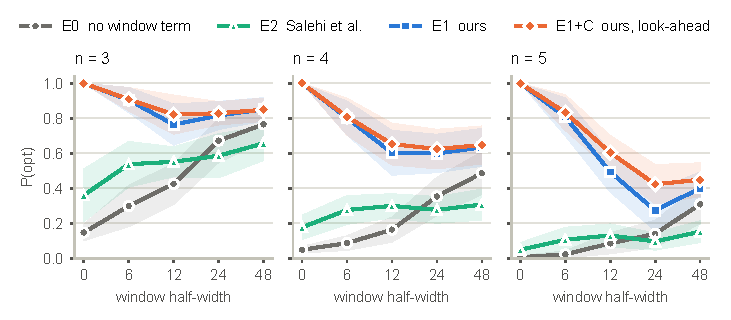
\includegraphics[width=\linewidth]{sa_tightness}
\caption{Simulated annealing $\Popt$ against the half-width of planted time windows (ordinal
axis), with weights re-tuned at every width; mean over 20 instances with 95\% t-interval bands.
At width 0 only the planted route is feasible.}\label{fig:tightness}
\end{figure}

% source: results/sa_tightness_summary.txt
Figure~\ref{fig:tightness} varies the window width. At width 0 only the planted route is
feasible, and E1 and E1+C find it in every read ($\Popt=1.000$ at every $n$, against 0.361, 0.178
and 0.050 for E2): windows of zero width make the bounds tight, a best case for a bound-based
penalty. As the windows loosen the advantage narrows but persists; at width 48 and $n=5$, E1+C
reaches 0.450 and E1 0.401, against 0.309 for E0 and 0.153 for E2. Each of E1 and E1+C has a
higher mean $\Popt$ than both E0 and E2 in all 15 combinations of width and size, whereas E2
beats E0 only at widths up to 12.

\subsection{QAOA}\label{sec:res-qaoa}
% source: results/qaoa_grid_summary.txt, "P(opt) minus E0's, paired per instance" rows, p = 1, 5, 12
\begin{table}[t]
\caption{QAOA: $\Popt$ minus E0's, paired per instance (mean $\pm$ 95\% CI), at depths
$p = 1, 5, 12$. 50 fresh instances per row (20 for the X mixer at $n=4$).}\label{tab:qaoa}
\centering\small\setlength{\tabcolsep}{5pt}
\begin{tabular}{llllll}
\toprule
Mixer & $n$ & Enc. & $p=1$ & $p=5$ & $p=12$\\
\midrule
XY & 3 & E1   & $+0.049\pm0.032$ & $+0.100\pm0.066$ & $+0.166\pm0.094$\\
   &   & E1+C & $+0.064\pm0.030$ & $+0.177\pm0.080$ & $+0.201\pm0.104$\\
   & 4 & E1   & $-0.002\pm0.005$ & $+0.029\pm0.023$ & $+0.072\pm0.073$\\
   &   & E1+C & $+0.003\pm0.003$ & $+0.087\pm0.038$ & $+0.217\pm0.071$\\
   & 5 & E1   & $+0.000\pm0.000$ & $+0.019\pm0.007$ & $+0.075\pm0.034$\\
   &   & E1+C & $+0.001\pm0.000$ & $+0.028\pm0.012$ & $+0.094\pm0.043$\\
\midrule
X  & 3 & E1   & $-0.008\pm0.002$ & $+0.026\pm0.010$ & $+0.197\pm0.052$\\
   &   & E1+C & $-0.011\pm0.004$ & $+0.057\pm0.020$ & $+0.231\pm0.054$\\
   & 4 & E1   & $-0.000\pm0.000$ & $+0.003\pm0.008$ & $+0.045\pm0.049$\\
   &   & E1+C & $-0.000\pm0.000$ & $+0.014\pm0.013$ & $+0.124\pm0.063$\\
\bottomrule
\end{tabular}
\end{table}

\begin{figure}[t]
\centering
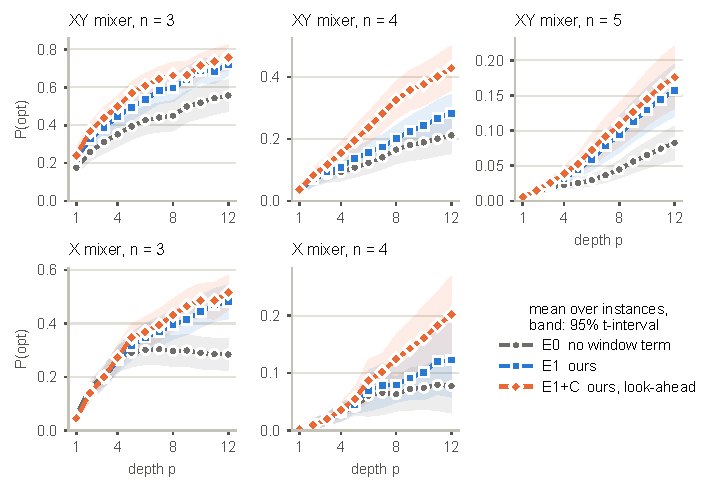
\includegraphics[width=\linewidth]{qaoa_depth}
\caption{QAOA $\Popt$ against depth: mean over 50 fresh instances (20 for the X mixer at
$n = 4$) with 95\% t-interval bands. Each panel has its own vertical scale.}\label{fig:depth}
\end{figure}

% source: results/qaoa_grid_summary.txt
Table~\ref{tab:qaoa} and Fig.~\ref{fig:depth} show the QAOA results. With the XY mixer, E1+C's
paired gain over E0 is positive at every depth and size and grows with depth, through $p=12$ at
$n=4,5$ and up to $p=8$ at $n=3$; at $p=12$ its interval excludes zero for every $n$. There E1+C
reaches $\Popt$ 0.758, 0.429 and 0.176 at $n=3,4,5$, against 0.556, 0.212 and 0.083 for E0 and
0.0800, 0.0097 and 0.0009 for a uniform sample of the XY mixer's states. E1's gains are smaller,
and at $n=4$ its interval at $p=12$ includes zero ($+0.072\pm0.073$). With the X mixer both
encodings lose slightly up to depth 3, presumably because the penalty terms make the shallow
landscape harder to optimise, and gain from $p=5$ on. The probability of an on-time route gains even
more: at $n=5$ and $p=12$ E1+C puts 0.556 of it on on-time routes, against 0.229 for E0.

Where does the gain come from? Instances whose TSP optimum is late are the obvious beneficiaries,
since there E0's cheapest route is infeasible. At $n=4$ (XY, $p=12$) these 10 instances carry
91\% of E1's gain. E1+C, however, also gains on the 40 instances whose TSP optimum is on time
($+0.180\pm0.075$), presumably because penalising cheap infeasible routes widens the energy gap
above the optimum even when the optimum is the cheapest route overall. With the XY mixer the
share of ground states that are optimal, the limit of $\Popt$ as $p\to\infty$ for a unique ground
state but not a bound at finite depth, rises at $n=5$ from 32\% for E0 to 64\% for E1 and 85\% for
E1+C.

\subsection{Circuit Cost}\label{sec:res-cost}
% source: qubits and X-mixer ZZ terms from results/sa_up_summary.txt (same instances and values as
% results/resources.txt, qubits to one decimal); XY-mixer ZZ terms from results/resources.txt
\begin{table}[tb]
\caption{Qubits and two-qubit (ZZ) terms per QAOA layer at $n=3,4,5$, mean over the 20
evaluation instances. Every nonzero off-diagonal QUBO entry is one ZZ rotation. E2 and E2-UP are
not run with QAOA, so they have no XY count.}\label{tab:resources}
\centering\small\setlength{\tabcolsep}{4pt}
\begin{tabular}{lrrrrrrrrr}
\toprule
 & \multicolumn{3}{c}{Qubits} & \multicolumn{3}{c}{ZZ, X mixer} & \multicolumn{3}{c}{ZZ, XY mixer}\\
\cmidrule(lr){2-4}\cmidrule(lr){5-7}\cmidrule(lr){8-10}
Enc. & 3 & 4 & 5 & 3 & 4 & 5 & 3 & 4 & 5\\
\midrule
E0    &  9.0 &  16.0 &  25.0 &  30.0 &   84.0 &  180.0 & 21.0 & 60.0 & 130.0\\
E1    &  9.0 &  16.0 &  25.0 &  30.0 &   84.0 &  180.0 & 21.0 & 60.0 & 130.0\\
E1+C  &  9.0 &  16.0 &  25.0 &  32.7 &   94.3 &  192.2 & 23.7 & 70.3 & 142.2\\
E2    & 60.5 & 102.4 & 165.7 & 875.0 & 2931.9 & 8773.9 & -- & -- & --\\
E2-UP & 29.0 &  60.0 & 111.2 & 348.7 & 1584.5 & 5660.4 & -- & -- & --\\
\bottomrule
\end{tabular}
\end{table}

% source: results/resources.txt, results/sa_up_summary.txt, results/pruning_check.txt
Table~\ref{tab:resources} gives the circuit cost. E1 needs exactly
E0's qubits and two-qubit terms with either mixer, as Sect.~\ref{sec:e1} predicts. E1+C adds the
$(k,k+2)$ couplings, 192.2 instead of 180.0 $ZZ$ terms per layer at $n=5$ with the X mixer (9\%
more on average over the instances of Table~\ref{tab:pruning}). E2 needs 165.7 qubits and 8773.9
$ZZ$ terms at $n=5$, and E2-UP, which drops the slack registers but keeps the waiting-time
registers, needs 111.2 and 5660.4. The XY mixer removes the row constraint from the cost
Hamiltonian, so our encodings need fewer $ZZ$ terms with it (130.0 instead of 180.0 at $n=5$), at
the price of $n^2$ $XY$ rotations per layer in the mixer.

% ---------------------------------------------------------------------------------------------
\section{Limitations}\label{sec:limits}
% source: results/qaoa_grid_summary.txt, results/qaoa_grid_edge.txt, grid.py docstring
Our quantum results come from exact, noiseless simulation of at most 25 qubits ($n\le5$); we
did not run hardware, model noise or sample finite shots, and the classical pruning analysis
reaches only $n=9$. E1 is sound but not complete, and the share of instances whose ground state is the optimum
falls with $n$ (Sect.~\ref{sec:res-pruning}); the QAOA set's 64\% for E1 at $n=5$ and
Table~\ref{tab:pruning}'s 46.5\% differ in weights and instances. The two baselines run only under simulated
annealing because their qubit counts are beyond exact simulation; E2's tuned window term was off
at $n=5$, and E2-UP is only one of several ways to apply unbalanced penalization. The X-mixer
weights chose the edge of the tuning grid, but re-tuning beyond it improves the tuning objective
by at most 0.007. We study one vehicle, no separate service times, integer metric travel times
and generated instances, and we compare with Rezk and Gora's penalty formulas only, not with
their coarsening and annealing pipeline.

% ---------------------------------------------------------------------------------------------
\section{Conclusion}\label{sec:conclusion}
Time windows need not cost qubits. Earliest-arrival bounds computed classically turn the windows
into penalties that sit on couplings the distance term already has, and because they are lower
bounds they never penalise a feasible route. E1 therefore has the window-free encoding's exact
circuit cost, and E1+C buys more pruning for a few percent more two-qubit terms. In exact QAOA
simulation with the XY mixer, E1+C raises the probability of the optimal route at every depth
and size we tested, and under simulated annealing both encodings beat a slack-qubit encoding and
its slack-free unbalanced-penalization variant with a fraction of their qubits. Next steps are
larger instances on approximate simulators and hardware, permutation-preserving
mixers~\cite{hadfield2019qaoa}, and the multi-vehicle CVRPTW~\cite{rezk2026gnn}.

% ---------------------------------------------------------------------------------------------
\subsubsection*{Disclosure of Interests.} The author has no competing interests to declare that
are relevant to the content of this article.

\subsubsection*{Use of AI Tools.} In line with Springer Nature's policy on AI-assisted research,
we disclose that AI assistants were used throughout this work: to
search and summarise the literature, to write and review the experiment code, and to draft the
text of this paper from the code, the saved results and the author's notes. The author checked
every equation, number and citation against the code and the saved results and takes full
responsibility for the content.


\bibliographystyle{splncs04}
\bibliography{refs}

\end{document}
